\documentclass[10pt]{article}
\usepackage[margin=1.0in]{geometry} % Please keep the margins at 1.5 so that there is space for grader comments.
\usepackage{amsmath,amsthm,amssymb,tikz}

\begin{document}
\begin{center}\Large Math 492 Quantam Physics Problem\end{center}
\begin{center}\large Ryan Toepfer and Carter Ronald\end{center}

\section{Problem Statement}
We have set out to analyze how the parameters of quantam systems govern how the state of the system changes over time.

\section{Axioms and Definitions}

Definition 2.1) A complex $A$ matrix is \textbf{skew hermitian} iff its transpose conjugate is equal to $-A$.
Therefore, all $2\times2$ skew hermitian matricies fit the form
\begin{center}
$\begin{pmatrix}ai&b+ci\\-b+ci&di\end{pmatrix}$
or alternatively, 
$\begin{pmatrix}ai&\beta\\-\bar\beta&di\end{pmatrix}$
\end{center}

Axiom 2.2) The state of a quantam system can be described entirely by $\begin{pmatrix}x\\y\end{pmatrix}$, where $x,y$ are complex numbers. 

Axiom 2.3) Two quantam states are considered the same if one is a multiple of another, i.e. $\begin{pmatrix}x\\y\end{pmatrix}=\alpha\begin{pmatrix}v\\w\end{pmatrix}$ for any $x,y,\alpha,v,w\in\mathbb C$, means both states are the same.
Therefore any state $\begin{pmatrix}x\\y\end{pmatrix}$ can be represented as a ratio $z=x/y$.

Axiom 2.4) The function describing the state of a quantam system at time $t$ is the solution to the ODE
\begin{center}$
\dot{\begin{pmatrix}x\\y\end{pmatrix}}=A\begin{pmatrix}x\\y\end{pmatrix}
$\end{center}
where $A$ is a skew hermation matrix.

\section{Initial Results}
Combining Axiom 2.4 with the general form of a $2\times2$ skew hermation matrix gives
\begin{center}
$\dot{\begin{pmatrix}x\\y\end{pmatrix}}=\begin{pmatrix}ai&\beta\\-\bar\beta&di\end{pmatrix}\begin{pmatrix}x\\y\end{pmatrix}$
or $\begin{cases}\dot x=aix+\beta y\\\dot y=-\bar\beta x+diy\end{cases}$
\end{center}
So if you consider $z=y/x$, and its derivative, then we get the following new equation
\begin{align*}
\dot z&=\frac{\dot yx-y\dot x}{x^2}\\
\dot z&=\frac{(-\bar\beta x+diy)x-y(aix+\beta y)}{x^2}\\
\dot z&=\frac{-\bar\beta x^2+diyx-aixy-\beta y^2}{x^2}\\
\dot z&=-\bar\beta+diz-aiz-\beta z^2
\end{align*}
From here we can make assumptions to make this easier to solve

\section{Assume $\beta=0, d=-a, a\neq0$}

Adding these assumptions to our initial result gives:
\begin{align*}
\dot z&=-2aiz
\end{align*}
Now we can define $f,g$ as the real and complex parts of $z$ respectively
\begin{align*}
\dot f+i\dot g&=-2ai(f+ig)\\
\dot f+i\dot g&=-2aif+2ag\\
\end{align*}
Giving the system:
\begin{align*}
\begin{cases}\dot f=2ag\\\dot g=-2af\end{cases}\\
\therefore \ddot f=2a\dot g\\
\ddot f=-4a^2f\\
\ddot f+4a^2f=0\\
\lambda^2+4a^2=0\\
\lambda^2=-4a^2\\
\lambda = \pm\sqrt{-4a^2} = \pm2ai\\
\end{align*}
So the solution is
\begin{align*}
f&=c_1e^0\cos(2at)+c_2e^0\sin(2at)\\
f&=c_1\cos(2at)+c_2\sin(2at)\\
\therefore \dot f&=-c_12a\sin(2at)+c_22a\cos(2at)
\end{align*}
pluggint $f$ into our equation for $\dot f$ gives $g$: 
\begin{align*}
\dot f&=2ag\\
-c_12a\sin(2at)+c_22a\cos(2at)&=2ag\\
-c_1\sin(2at)+c_2\cos(2at)&=g\\
\end{align*}
As a vector gives:
\begin{align*}
\begin{pmatrix}f\\g\end{pmatrix}=
\begin{pmatrix}c_1\cos(2at)+c_2\sin(2at)\\-c_1\sin(2at)+c_2\cos(2at)\end{pmatrix}
\end{align*}

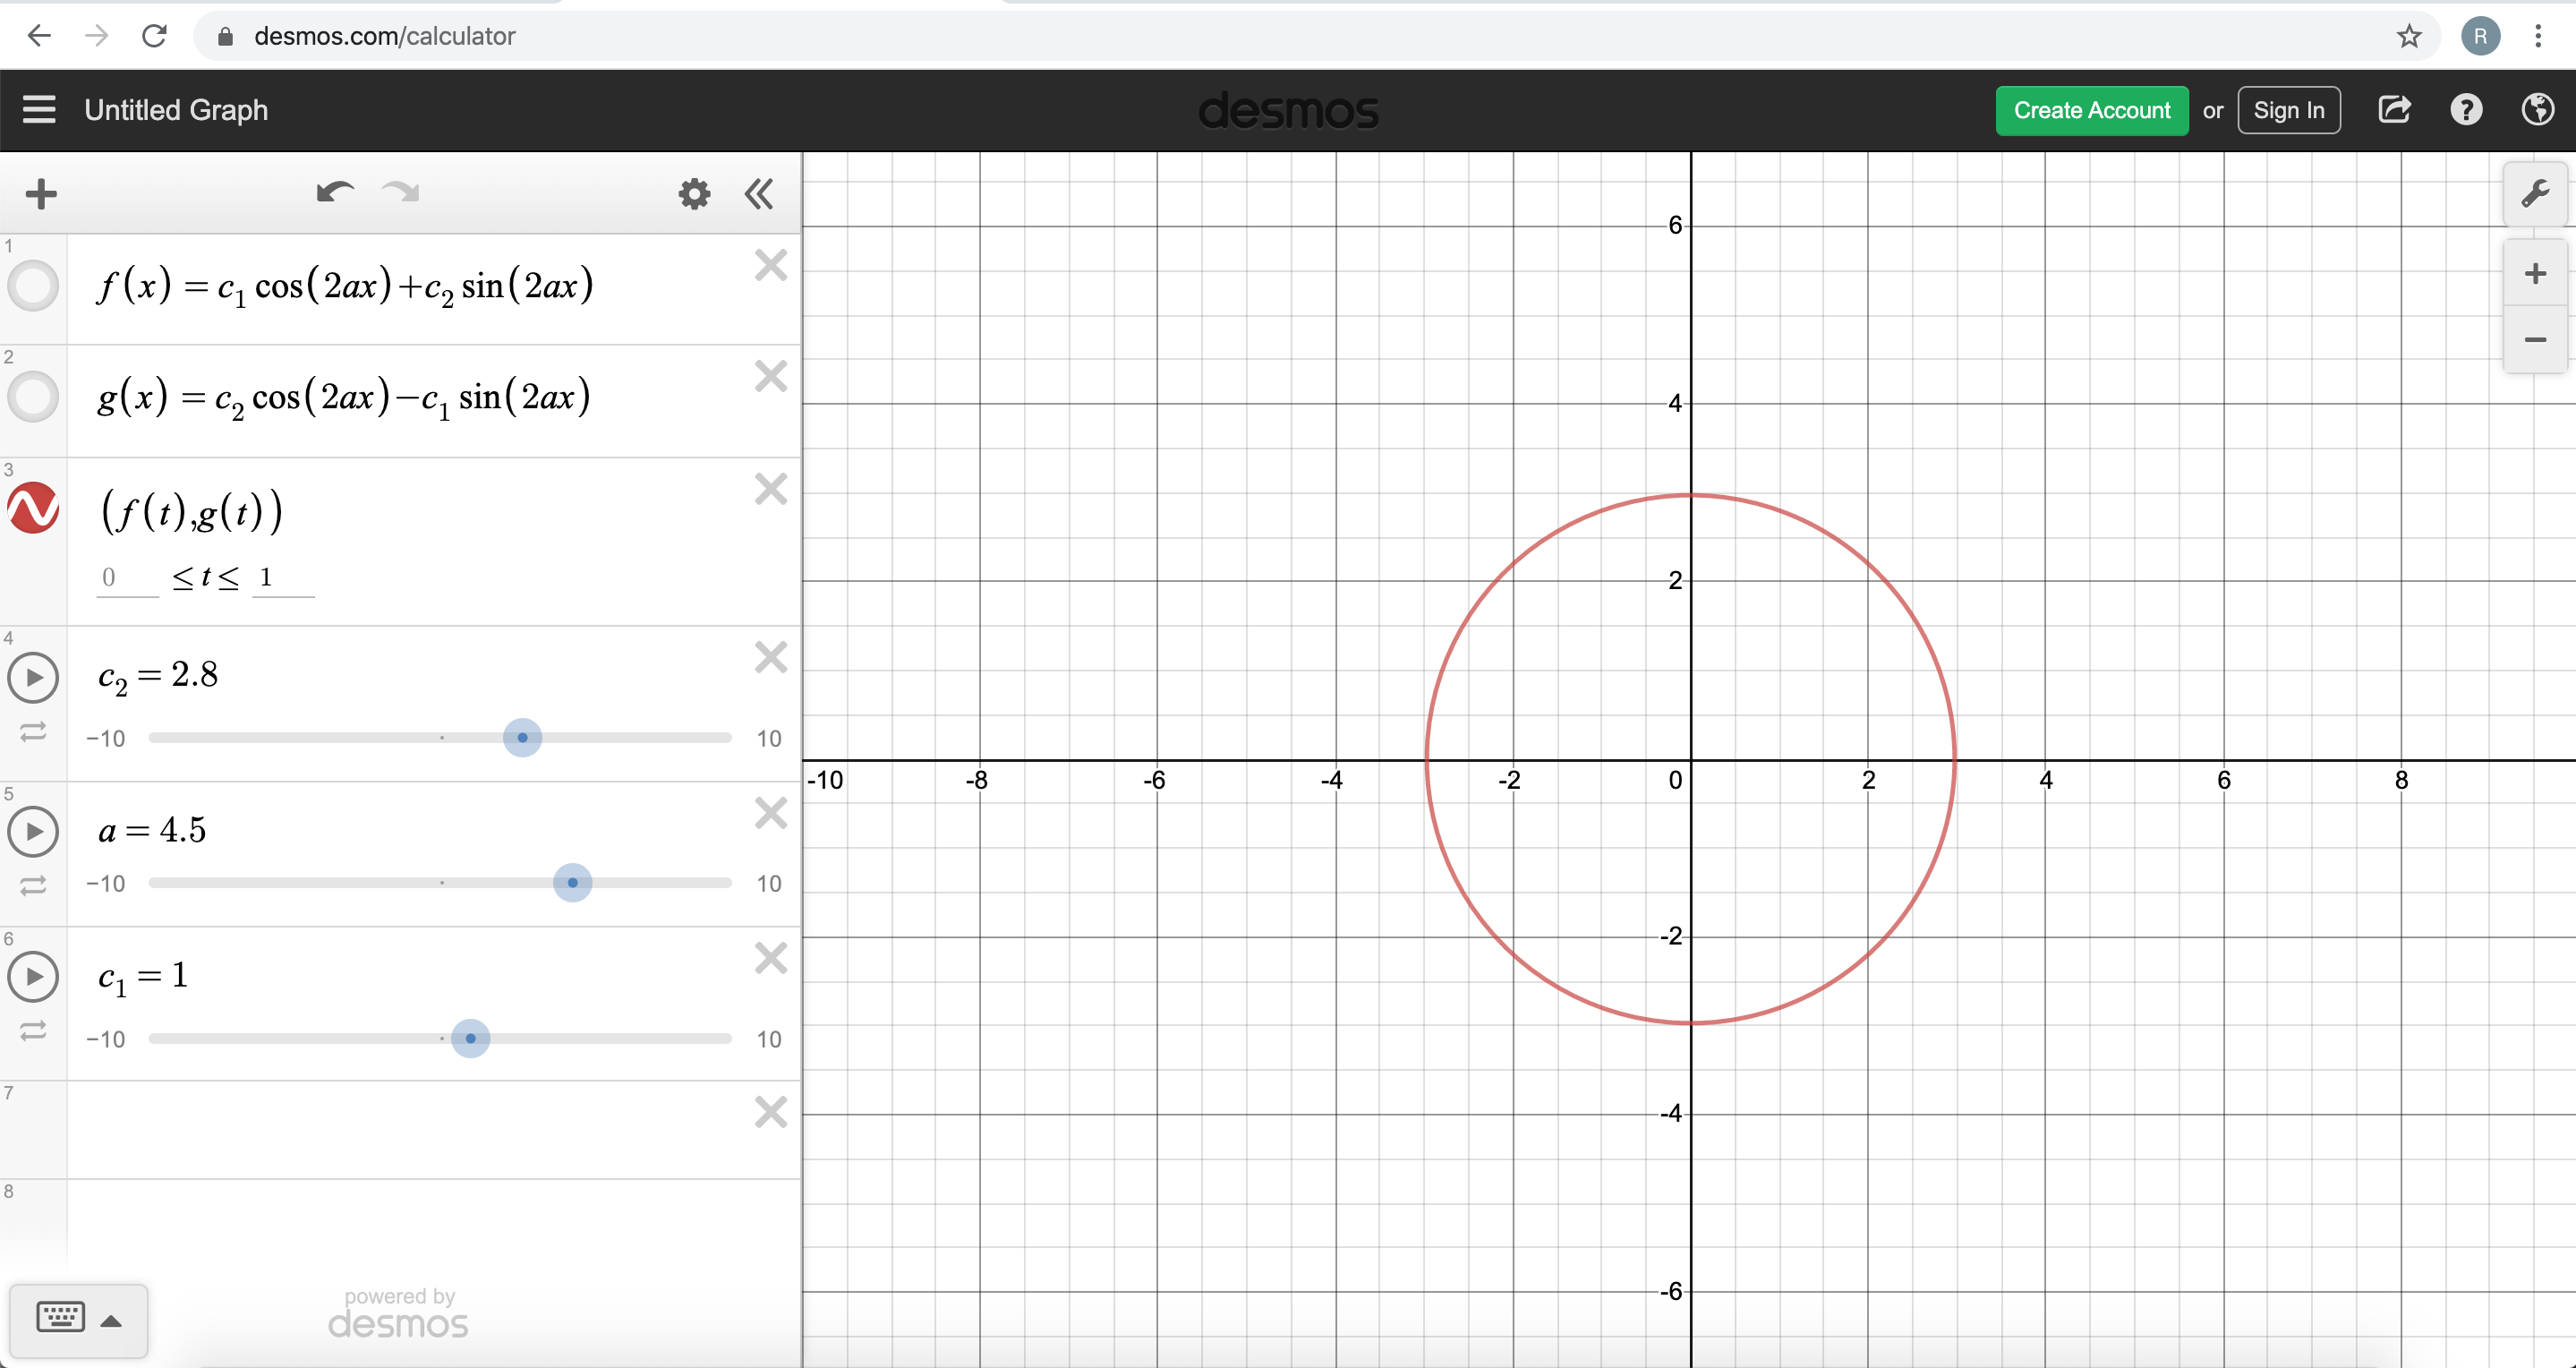
\includegraphics[width=\textwidth]{Figure1}
Changing $c_1$ and $c_2$ affects the size of the circle.
Changing $a$ only affects the paramaterization.

\end{document}